% pdflatex -shell-escape template_cdc.tex

\documentclass[a4paper,oneside]{article}

\usepackage[frenchb]{babel}
\usepackage[utf8]{inputenc}
\usepackage[T1]{fontenc}
\usepackage{graphicx}
\usepackage{amssymb} 
\usepackage{amsmath}
\usepackage{hyperref}
\usepackage{fullpage}
\usepackage{epstopdf}


%%%%%%%%%%%%%%%%%%%%%%%%%

\newcommand{\mytitle}{Projet Puissance X - Cahier des charges}
\title{\mytitle } 

%%%%%%%%%%%%%%%%%%%%%%%%%

\makeatletter

\usepackage{fancyhdr}
\pagestyle{fancyplain}
\fancyhf{}
\renewcommand{\headrulewidth}{0pt}
\renewcommand{\footrulewidth}{0.5pt}
\lfoot{\mytitle}
\cfoot{\@date}
\rfoot{page \thepage / \pageref{fin}}

\author{Benjamin CLETON, Clement ANSEL et Matthieu LANIESSE}

\date{29 mai 2017}


%%%%%%%%%%%%%%%%%%%%%%%%%


\begin{document}

\maketitle

\thispagestyle{fancyplain}


%%%%%%%%%%%%%%%%%%%%%%%%%

\section{Renseignements}

\paragraph{Nom du projet :}
Puissance X

\paragraph{Objet :}
Développement d'un jeu en tour par tour contre un ordinateur

\paragraph{Maître d'ouvrage :}
Benjamin CLETON, Clement ANSEL, Matthieu LANIESSE

\paragraph{Maître d'oeuvre : }
Benjamin CLLETON, Clement ANSEL, Matthieu LANIESSE

\paragraph{Date de début :}
29 mai 2017

\paragraph{Date de fin :}
16 juin 2017


%%%%%%%%%%%%%%%%%%%%%%%%%

\newpage

\section{Définition du besoin}

\paragraph{Contexte général\\}
Benjamin, Clément et Matthieu sont 3 étudiants qui ont pour projet de créer un jeu avec une intelligence artificielle dans le cadre de leurs études.
Nostalgique de leur enfance, l'idée d'un puissance X leur est venu comme une évidence.


\paragraph{Besoins et priorités\\}
Le besoin principal est de pouvoir jouer au puissance X de plusieurs manières :
\begin{itemize}
	\item Ordinateur versus ordinateur
	\item Joueur versus ordinateur
	\item Joueur versus Joueur
	\item Choix de la taille du plateau
\end{itemize}

En ce qui concerne les priorités du puissance X, voici  un ordre de classement :
\begin{itemize}
	\item Interface
	\item Logique du jeu
	\item Intelligence Artificielle
	\item Paramètres
	\item Règles
	\item Score
\end{itemize}


%%%%%%%%%%%%%%%%%%%%%%%%%

\newpage

\section{Spécifications}

\begin{itemize}
    \item Jeu fonctionnant sur tous les ordinateurs vendus dans le commerce.
    \item fonctionnalités du Puissance X :
        \begin{itemize}
        	\item Choisir le nombre de pions alignés permettant la victoire
        	\item Choisir la taille de la grille
            	\item Placer des jetons dans une grille
            	\item Afficher les scores
            	\item Choisir un Pseudonyme 
            	\item Choisir un mode de jeu
            	\item Choisir un degré de difficulté
		\item Choisir une IA en particulier
            	\item Implémentation d'un son après un coup joué
        \end{itemize}
    \item interface utilisateur :
        \begin{itemize}
            	\item Affichage de la grille de jeu en deux dimensions
            	\item Affichage des Pseudonymes et des joueurs
            	\item Affichage des boutons de réglages
            	\item Affichage d'un menu après fin d'une partie
        \end{itemize}
    \item performances demandées :
        \begin{itemize}
            	\item Niveaux de difficultés différent pour chaque IA
        \end{itemize}

\end{itemize}


%%%%%%%%%%%%%%%%%%%%%%%%%

\newpage

\appendix

\section{Livrables}

\begin{itemize}
    \item Jeu déployé sur tout les ordinateurs vendu dans le commerce
    \item code source programmé avec la bibliothèque open source Swing(Java)
\end{itemize}







\section{Maquettes}

\paragraph{Page du Menu Principal}

~\\

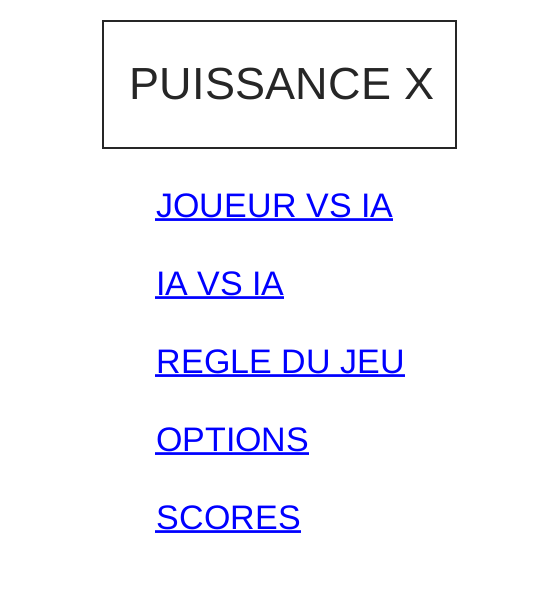
\includegraphics[width=9cm]{image2.png}

\paragraph{Page de Jeu}

~\\

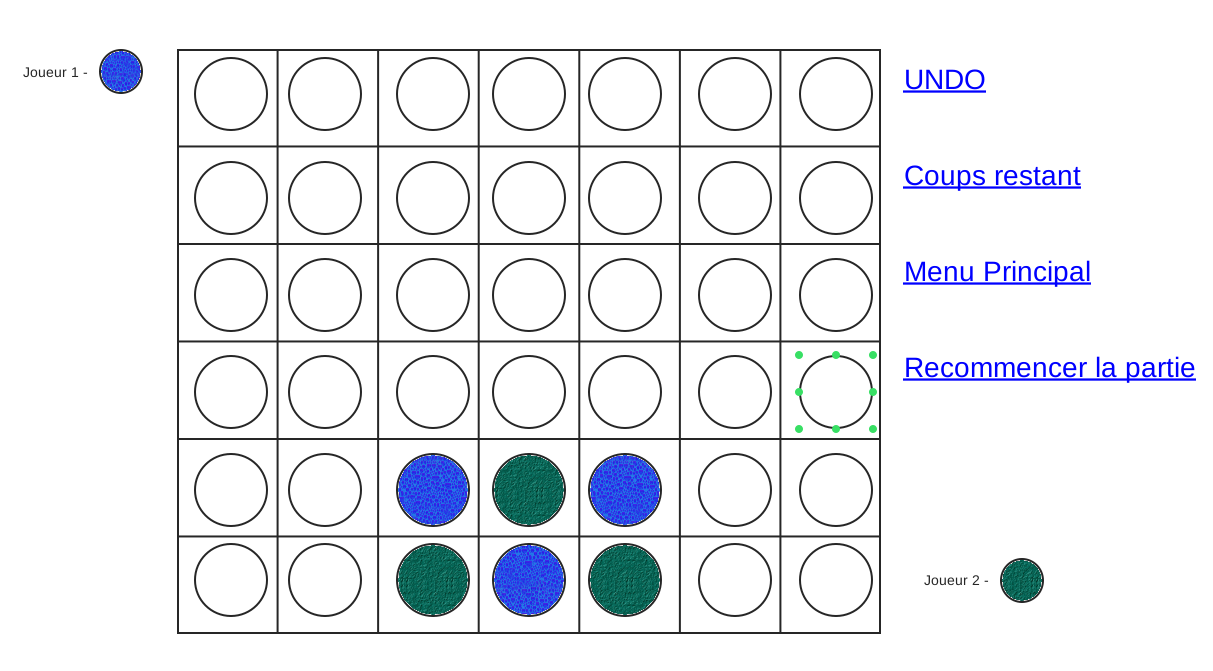
\includegraphics[width=13cm]{image1.png}




%%%%%%%%%%%%%%%%%%%%%%%%%

\label{fin}

\end{document}


